% === B01 - SIMD Saturacion Empaquetado Extension Mascaras ===
% David Alejandro Gonzalez Marquez
% dmarquez@dc.uba.ar / fokerman@gmail.com
% https://github.com/fokerman/Orga2Course

\documentclass[aspectratio=169]{beamer}
% \documentclass[handout]{beamer}

% % % Packages
\usepackage[sfdefault]{AlegreyaSans}
\usepackage{inconsolata}
\usepackage{multicol}
\usepackage{multirow}
\usepackage[spanish]{babel}
\usepackage[utf8]{inputenc} 
\usepackage{enumerate}
\usepackage{color}
\usepackage{xcolor}
\usepackage[absolute,overlay]{textpos}
  \setlength{\TPHorizModule}{1mm}
  \setlength{\TPVertModule}{1mm}
\usepackage{framed}
\usepackage{mfirstuc} % para poner en mayusculas la primer letra
\usepackage{xspace} % para crear espacios en comandos 
\usepackage{pbox}
\usepackage{tikz}
\usepackage{mathabx}

% % % Beamer config
\usetheme{Pittsburgh}
\usecolortheme[rgb={1,0.48,0.0}]{structure}
\setbeamercolor{block title}{fg=white,bg=verdeuca}
\xdefinecolor{verdeuca}{rgb}{0.0,0.48,0.54}
\xdefinecolor{naranjauca}{rgb}{1,0.48,0.0}
\setbeamercolor{palette quaternary}{fg=white,bg=verdeuca}
\setbeamertemplate{title page}[default][colsep=-4bp, rounded=true] % remove title shadow
\setbeamertemplate{frametitle}[default][colsep=-2bp, shadow=false] % remove frame title shadow
\setbeamertemplate{navigation symbols}{} % remove navigation symbols
\beamertemplatenavigationsymbolsempty

% % % Colors
\definecolor{AzulClaro}{rgb}{.31,.506,.741}
\definecolor{Gris}{gray}{0.8}
\definecolor{Celeste}{rgb}{.255,.41,.884}
\definecolor{Rojo}{rgb}{1, 0, 0}
\definecolor{a}{rgb}{0.0, 0.53, 0.74}
\definecolor{r}{rgb}{0.89, 0.0, 0.13}
\definecolor{v}{rgb}{0.0, 0.5, 0.0}
\definecolor{y}{rgb}{0.0, 0.5, 0.5}

% % % Rename
\newcommand{\tab}[0]{\hspace{15pt}}

% % % Blocks
\setbeamercolor{block body}{fg=black, bg=black!10}
\setbeamercolor{block title}{fg=black, bg=black!20}
\setbeamercolor{coloredboxstuffNaranja}{fg=naranjauca,bg=black!10} %% PARA LOS BOX
\setbeamercolor{coloredboxstuffVerde}{fg=verdeuca,bg=black!10} %% PARA LOS BOX

% % % Start

\title{\Huge SIMD Parte 1}
\subtitle{Saturación, Empaquetado, Extensión y Mascaras}
      
\author{David Alejandro González Márquez}
\institute{Departamento de Computación\\
Facultad de Ciencias Exactas y Naturales\\
Universidad de Buenos Aires}
\date{}

\begin{document}

\begin{frame}[plain]
    \titlepage 
\end{frame}

\begin{frame}[fragile]
    \frametitle{Introducción}
    \begin{itemize}
    \setlength\itemsep{0.5cm}
    \large
     \item[-] Vamos a resolver algoritmos utililzando \textbf{instrucciones vectoriales}.
     \item[-] Debemos \textbf{conocer} las instrucciones que tenemos disponibles.
     \item[-] y las \textbf{técnicas} para pensar algoritmos desde la operatoria vectoriales.
    \end{itemize}
\end{frame}

\begin{frame}[fragile]
    \frametitle{Registros y tipos de datos}
    \large
    \begin{itemize}
    \setlength\itemsep{0.7cm}
     \item[-] Registros:\\
     \vspace{0.2cm}
     \hspace{2cm} \texttt{XMM0} a \texttt{XMM15} de 128 bits (16 bytes)
     \item[-] Tipos de datos:\\
     \vspace{0.2cm}
     \hspace{2cm} Enteros: \texttt{8}, \texttt{16}, \texttt{32}, \texttt{64} y \texttt{128}.\\
     \vspace{0.2cm}
     \hspace{2cm} Float: \texttt{32} (Float) y \texttt{64} (Double).
    \end{itemize}
\end{frame}


\begin{frame}[fragile,t]
    \frametitle{Operaciones Load/Store}
    \begin{center}
    \begin{tabular}{ll|l}
    \hline
    \texttt{MOV\color{v}{D}}              & \texttt{MOV\color{v}{Q}} & Move Doubleword/Quadword \\
    \texttt{MOV\color{v}{SS}}             & \texttt{MOV\color{v}{SD}} & Moves a 32bits Single FP/64bits Double FP \\
    \hline
    \texttt{MOV\color{v}{DQ}\color{a}{A}} & \texttt{MOV\color{v}{DQ}\color{a}{U}} & Moves aligned/unaligned double quadword \\
    \texttt{MOV\color{a}{A}\color{v}{PS}} & \texttt{MOV\color{a}{U}\color{v}{PS}} & Moves 4 aligned/unaligned 32bit singles \\
    \texttt{MOV\color{a}{A}\color{v}{PD}} & \texttt{MOV\color{a}{U}\color{v}{PD}} & Moves 2 aligned/unaligned 64bit doubles \\
    \hline
    \pause
    \end{tabular}
    \end{center}
    \vspace{-0.3cm}
    Ejemplo:\\
    \vspace{-0.5cm}
    \begin{center}
    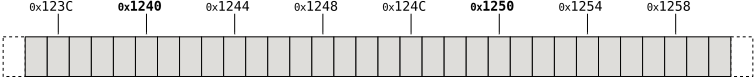
\includegraphics[scale=0.6]{img/inst_mov.pdf}
    \end{center}
    \pause
    \begin{tabular}{lll}
    \normalsize \texttt{MOVD [0x123C], xmm0 }   & { \hspace{0.2cm} \large \checkmark } & \normalsize \texttt{[0x123C]} $\leftarrow$ \texttt{xmm0(32:0)} \\
    \pause
    \normalsize \texttt{MOVQ xmm0, [0x1245] }   & { \hspace{0.2cm} \large \checkmark } & \normalsize \texttt{xmm0(64:0)} $\leftarrow$ \texttt{[0x1245]} \\
    \pause
    \normalsize \texttt{MOVDQA xmm0, [0x1245] } & { \hspace{0.2cm} \Large $\times$}    & \normalsize Error dirección no alineada. \\
    \pause
    \normalsize \texttt{MOVDQA [0x1250], xmm0 } & { \hspace{0.2cm} \large \checkmark } & \normalsize \texttt{[0x1250]} $\leftarrow$ \texttt{xmm0(128:0)} \\
    \pause
    \normalsize \texttt{MOVSS xmm0, [0x1248] }  & { \hspace{0.2cm} \large \checkmark } & \normalsize \texttt{xmm0(32:0)} $\leftarrow$ \texttt{[0x1248]} \small ; sobre punto flotante \\
    \pause
    \normalsize \texttt{MOVUPS [0x1258], xmm0 } & { \hspace{0.2cm} \large \checkmark } & \normalsize \texttt{[0x1258]} $\leftarrow$ \texttt{xmm0(128:0)} \small ; sobre punto flotante \\
    \end{tabular}
    
\end{frame}
%\large \checkmark \Large $\times$

\begin{frame}[fragile,t]
    \frametitle{Operaciones Load/Store}
    \begin{center}
    \begin{tabular}{ll|l}
    \hline
    \texttt{PMOV\color{a}{S}\color{black}{X}\color{v}{BW}} & \texttt{PMOV\color{a}{Z}\color{black}{X}\color{v}{BW}} & packed sign/zero extension byte to word\\
    \texttt{PMOV\color{a}{S}\color{black}{X}\color{v}{BD}} & \texttt{PMOV\color{a}{Z}\color{black}{X}\color{v}{BD}} & packed sign/zero extension byte to dword\\
    \texttt{PMOV\color{a}{S}\color{black}{X}\color{v}{BQ}} & \texttt{PMOV\color{a}{Z}\color{black}{X}\color{v}{BQ}} & packed sign/zero extension byte to qword\\
    \texttt{PMOV\color{a}{S}\color{black}{X}\color{v}{WD}} & \texttt{PMOV\color{a}{Z}\color{black}{X}\color{v}{WD}} & packed sign/zero extension word to dword\\ 
    \texttt{PMOV\color{a}{S}\color{black}{X}\color{v}{WQ}} & \texttt{PMOV\color{a}{Z}\color{black}{X}\color{v}{WQ}} & packed sign/zero extension word to qword\\
    \texttt{PMOV\color{a}{S}\color{black}{X}\color{v}{DQ}} & \texttt{PMOV\color{a}{Z}\color{black}{X}\color{v}{DQ}} & packed sign/zero extension word to dqword\\
    \hline
    \end{tabular}
    \end{center}
    \only<3->{Ejemplos:}
    \begin{textblock}{500}(5,50)
    \begin{tabular}{lll}
    \uncover<3->{ & \\ } % HACK 
    \uncover<4->{ \texttt{PMOVSXBD xmm0, xmm0}   & { \hspace{0.2cm} \large \checkmark} & \\ }
    \uncover<5->{ \texttt{PMOVZXWD xmm0, [data]} & { \hspace{0.2cm} \large \checkmark} & \\ }
    \uncover<6->{ \texttt{PMOVZXDQ xmm0, xmm1}   & { \hspace{0.2cm} \large \checkmark} & \\ }
    \uncover<7->{ \texttt{PMOVZXQD xmm0, xmm0}   & { \hspace{0.2cm} \Large $\times$}   & Instrucción invalida.\\ }
    \uncover<8->{ \texttt{PMOVSXBD [data], xmm0} & { \hspace{0.2cm} \Large $\times$}   & Modo de direccionamiento invalido.\\ }
    \end{tabular}
    \end{textblock}
    \begin{textblock}{500}(70,50) \only<4>{\includegraphics[scale=0.7]{img/inst_extend-layer1.pdf}} \end{textblock}
    \begin{textblock}{500}(70,50) \only<5>{\includegraphics[scale=0.7]{img/inst_extend-layer2.pdf}} \end{textblock}
    \begin{textblock}{500}(70,50) \only<6>{\includegraphics[scale=0.7]{img/inst_extend-layer3.pdf}} \end{textblock}
\end{frame}

% movhps movlps     - Moves 64bit value into top/bottom half of an xmm
% movhpd movlpd     - Moves top/bottom 64bit value to or from an XMM register
% movhlps           - Move Packed Single-Precision Floating-Point Values High to Low
% movlhps           - Move Packed Single-Precision Floating-Point Values Low to High
% movddup           - Move One Double FP and Duplicate
% movmskps          - Extract Packed Single-Precision Floating-Point Sign Mask
% maskmovdqu        - Store Selected Bytes of Double Quadword
% maskmovq          - Store Selected Bytes of Quadword
% maskmovdqu        - Moves 16 bytes based on sign bits of another XMM register
% pmovmskb          - Generates a 16bit Mask from the sign bits of each byte in an XMM register

\begin{frame}[fragile,t]
    \frametitle{Operaciones Aritméticas}
    \begin{center}
    \begin{tabular}{llll|l}
    \hline
    \texttt{PADD}\color{v}{\texttt{B}}  &  \texttt{PADD}\color{v}{\texttt{W}}  &  \texttt{PADD}\color{v}{\texttt{D}} & \texttt{PADD}\color{v}{\texttt{Q}} & Add Integer \\
    \texttt{PSUB}\color{v}{\texttt{B}}  &  \texttt{PSUB}\color{v}{\texttt{W}}  &  \texttt{PSUB}\color{v}{\texttt{D}} & \texttt{PSUB}\color{v}{\texttt{Q}} & Sub Integer \\
    \hline
    \texttt{PMUL}\color{orange}{\texttt{H}}\color{v}{\texttt{W}} &  \texttt{PMUL}\color{orange}{\texttt{L}}\color{v}{\texttt{W}} & & & Mul Integer Word \\
    \texttt{PMUL}\color{orange}{\texttt{H}}\color{v}{\texttt{D}} &  \texttt{PMUL}\color{orange}{\texttt{L}}\color{v}{\texttt{D}} & & & Mul Integer Dword \\
    \hline
    \texttt{PMIN\color{a}{S}\color{v}{B}} & \texttt{PMAX\color{a}{S}\color{v}{B}} & \texttt{PMIN\color{a}{U}\color{v}{B}} & \texttt{PMAX\color{a}{U}\color{v}{B}} & Max and Min Integer \\
    \texttt{PMIN\color{a}{S}\color{v}{W}} & \texttt{PMAX\color{a}{S}\color{v}{W}} & \texttt{PMIN\color{a}{U}\color{v}{W}} & \texttt{PMAX\color{a}{U}\color{v}{W}} & Max and Min Integer \\
    \texttt{PMIN\color{a}{S}\color{v}{D}} & \texttt{PMAX\color{a}{S}\color{v}{D}} & \texttt{PMIN\color{a}{U}\color{v}{D}} & \texttt{PMAX\color{a}{U}\color{v}{D}} & Max and Min Integer \\
    \hline
    \end{tabular}
    \end{center}
    \uncover<2->{Ejemplos:}
    \begin{textblock}{500}(5,55)
    \begin{tabular}{lll}
    \uncover<3->{ & \\ } % HACK 
    \uncover<3->{ \texttt{PADDD xmm0, xmm1}    & { \hspace{0.2cm} \large \checkmark} & \\ }
    \uncover<4->{ \texttt{PSUBW xmm0, [data]}  & { \hspace{0.2cm} \large \checkmark} & \\ }
    \uncover<5->{ \texttt{PMULLD xmm0, xmm1}   & { \hspace{0.2cm} \large \checkmark} & \\ }
    \uncover<6->{ \texttt{PMAXSW xmm0, [data]} & { \hspace{0.2cm} \Large \checkmark} & \\ }
    \uncover<7->{ \texttt{PMINSB [data], xmm0} & { \hspace{0.2cm} \Large $\times$  } & Modo de direccionamiento invalido.\\ }
    \end{tabular}
    \end{textblock}
    \begin{textblock}{500}(70,50) \only<3>{\includegraphics[scale=0.7]{img/inst_op2-layer1.pdf}} \end{textblock}
    \begin{textblock}{500}(70,50) \only<4>{\includegraphics[scale=0.7]{img/inst_op2-layer2.pdf}} \end{textblock}
    \begin{textblock}{500}(70,50) \only<5>{\includegraphics[scale=0.7]{img/inst_op2-layer3.pdf}} \end{textblock}
    \begin{textblock}{500}(70,50) \only<6>{\includegraphics[scale=0.7]{img/inst_op2-layer4.pdf}} \end{textblock}
\end{frame}


\begin{frame}[fragile,t]
    \frametitle{Operaciones Aritméticas}
    \vspace{0.5cm}
    \begin{center}
    \begin{tabular}{l|l}
    \hline
    \texttt{PABS}\color{v}{\texttt{B}}  & Absolute for 8 bit Integers \\
    \texttt{PABS}\color{v}{\texttt{W}}  & Absolute for 16 bit Integers \\
    \texttt{PABS}\color{v}{\texttt{D}}  & Absolute for 32 bit Integers \\
    \hline
    \end{tabular}
    \end{center}
    \uncover<2->{Ejemplos:}
    \begin{textblock}{500}(5,40)
    \begin{tabular}{lll}
    \uncover<2->{ & \\ } % HACK 
    \uncover<3->{ \texttt{PABSD xmm0, xmm0}   & { \hspace{0.2cm} \large \checkmark} & \\ }
    \uncover<4->{ \texttt{PABSD xmm0, [data]} & { \hspace{0.2cm} \large \checkmark} & \\ }
    \uncover<5->{ \texttt{PABSD [data], xmm0} & { \hspace{0.2cm} \Large $\times$} & Modo de direccionamiento invalido.\\ }
    \end{tabular}
    \end{textblock}
    \begin{textblock}{500}(70,50) \only<3-4>{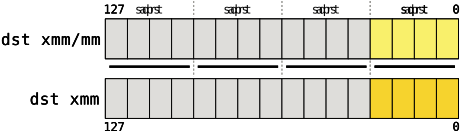
\includegraphics[scale=0.7]{img/inst_op1.pdf}} \end{textblock}
\end{frame}


\begin{frame}[fragile]
    \frametitle{Ejemplo}
    \begin{block}{Suma Uno}
    Dado un vector de $n$ enteros sin signo de 16 bits. Incrementa en 1 unidad cada uno y almacena el resultado en un vector de 16 bits.\\
    Considerar $n \equiv 0$ $(mod\ 8)$.\\
    \bigskip
    \verb|void suma1(uint16_t *vector, uint16_t *resultado, uint8_t n)|
    \end{block}
\end{frame}

\begin{frame}[fragile]
    \frametitle{Suma Uno}
    \scriptsize
    \begin{verbatim}
    section .rodata
    uno: times 8 dw 1

    section .text

    suma1: ; rdi = vector, rsi = resultado, dx = n
    \end{verbatim}
    \vspace{-0.8cm} \pause
    \begin{verbatim}
        push rbp
        mov rbp,rsp
    \end{verbatim}
    \vspace{-0.8cm} \pause
    \begin{verbatim}
        movzx rcx, dx
        shr ecx, 3         ; divido por 8
    \end{verbatim}
    \vspace{-0.8cm} \pause
    \begin{verbatim}
        movdqu xmm8, [uno] ; xmm8 = | 1 | 1 | 1 | 1 | 1 | 1 | 1 | 1 |
    \end{verbatim}
    \vspace{-0.8cm} \pause
    \begin{verbatim}
        .ciclo:
    \end{verbatim}
    \vspace{-0.8cm} \pause
    \begin{verbatim}
            movdqu xmm0, [rdi] ; xmm0 = | d7 | d6 | d5 | d4 | d3 | d2 | d1 | d0 |
    \end{verbatim}
    \vspace{-0.8cm} \pause
    \begin{verbatim}
            paddw  xmm0, xmm8  ; xmm0 = |d7+1|d6+1|d5+1|d4+1|d3+1|d2+1|d1+1|d0+1|
    \end{verbatim}
    \vspace{-0.8cm} \pause
    \begin{verbatim}
            movdqu [rsi], xmm0
    \end{verbatim}
    \vspace{-0.8cm} \pause
    \begin{verbatim}
            add rdi, 16
            add rsi, 16
    \end{verbatim}
    \vspace{-0.8cm} \pause
    \begin{verbatim}
        loop .ciclo
        pop rbp
        ret 
    \end{verbatim}
\end{frame}

\begin{frame}[fragile]
    \frametitle{Ejemplo}
    \begin{block}{Suma Dos}
    Dado un vector de $n$ enteros con signo de 16 bits. Incrementa en 2 unidades cada uno y almacena el resultado en un vector de 32 bits.\\
    Considerar $n \equiv 0$ $(mod\ 8)$.\\
    \bigskip
    \verb|void suma2(int16_t *vector, int32_t *resultado, uint8_t n)|
    \end{block}
\end{frame}

\begin{frame}[fragile]
    \frametitle{Suma Dos}
    \scriptsize
    \begin{verbatim}
    section .rodata
    dos: times 4 dd 2

    section .text

    suma2: ; rdi = vector, rsi = resultado, dx = n
        push rbp
        mov rbp,rsp
    \end{verbatim}
    \vspace{-0.8cm} \pause
    \begin{verbatim}
        movzx rcx, dx
        shr ecx, 2         ; divido por 4
    \end{verbatim}
    \vspace{-0.8cm} \pause
    \begin{verbatim}
        movdqu xmm8, [dos] ; xmm8 = | 2 | 2 | 2 | 2 |
    \end{verbatim}
    \vspace{-0.8cm} \pause
    \begin{verbatim}
        .ciclo:
    \end{verbatim}
    \vspace{-0.8cm} \pause
    \begin{verbatim}
            pmovsxwd xmm0, [rdi]  ; xmm0 = | d3 | d2 | d1 | d0 |
    \end{verbatim}
    \vspace{-0.8cm} \pause
    \begin{verbatim}
            paddd  xmm0, xmm8     ; xmm0 = |d3+2|d2+2|d1+2|d0+2|
            movdqu [rsi], xmm0
            add rdi, 8
            add rsi, 16
        loop .ciclo
    \end{verbatim}
    \vspace{-0.8cm} \pause
    \begin{verbatim}
        pop rbp
        ret 
    \end{verbatim}
\end{frame}

\begin{frame}[fragile,t]
    \frametitle{Operaciones Aritméticas}
    \begin{center}
    \begin{tabular}{ll|l}
    \hline
    \texttt{PADD}\color{r}{\texttt{S}}\color{v}{\texttt{B}}                      & \texttt{PADD}\color{r}{\texttt{S}}\color{v}{\texttt{W}}                        & Add Int saturation            \\
    \texttt{PADD}\color{a}{\texttt{U}}\color{r}{\texttt{S}}\color{v}{\texttt{B}} & \texttt{PADD}\color{a}{\texttt{U}}\color{r}{\texttt{S}}\color{v}{\texttt{W}}   & Add Int unsigned saturation   \\
    \texttt{PSUB}\color{r}{\texttt{S}}\color{v}{\texttt{B}}                      & \texttt{PSUB}\color{r}{\texttt{S}}\color{v}{\texttt{W}}                        & Sub Int saturation            \\
    \texttt{PSUB}\color{a}{\texttt{U}}\color{r}{\texttt{S}}\color{v}{\texttt{B}} & \texttt{PSUB}\color{a}{\texttt{U}}\color{r}{\texttt{S}}\color{v}{\texttt{W}}   & Sub Int unsigned saturation   \\
    \hline
    \end{tabular}
    \end{center}
    \uncover<2->{Ejemplos:}
    \begin{textblock}{500}(5,40)
    \begin{tabular}{lll}
    \uncover<2->{ & \\ } % HACK 
    \uncover<3->{ \texttt{PADDSW xmm0, xmm0}    & { \hspace{0.2cm} \large \checkmark} & \\ }
    \uncover<4->{ \texttt{PSUBUSB xmm0, [data]} & { \hspace{0.2cm} \large \checkmark} & \\ }
    \uncover<5->{ \texttt{PSUBSW [data], xmm0}  & { \hspace{0.2cm} \Large $\times$} & Modo de direccionamiento invalido.\\ }
    \end{tabular}
    \end{textblock}
    \begin{textblock}{500}(70,45) \only<3>{\includegraphics[scale=0.7]{img/inst_op2-layer5.pdf}} \end{textblock}
    \begin{textblock}{500}(70,45) \only<4>{\includegraphics[scale=0.7]{img/inst_op2-layer6.pdf}} \end{textblock}
\end{frame}

\begin{frame}[fragile]
    \frametitle{Ejemplo}
    \begin{block}{Suma Tres}
    Dado un vector de $n$ enteros con signo de 16 bits. Incrementa en 3 unidades cada uno y almacena el resultado en el mismo vector de forma saturada.\\
    Considerar $n \equiv 0$ $(mod\ 8)$.\\
    \bigskip
    \verb|void suma3(int16_t *vector, uint8_t n)|
    \end{block}
\end{frame}

\begin{frame}[fragile]
    \frametitle{Suma Tres}
    \scriptsize
    \begin{verbatim}
    section .rodata
    tres: times 8 dw 3

    section .text

    suma3: ; rdi = vector, rsi = n
        push rbp
        mov rbp,rsp
        movzx rcx, si
        shr ecx, 3              ; divido por 8
        movdqu xmm8, [tres]     ; xmm8 = | 3 | 3 | 3 | 3 | 3 | 3 | 3 | 3 |
    \end{verbatim}
    \vspace{-0.8cm} \pause
    \begin{verbatim}
        .ciclo:
            movdqu xmm0, [rdi]  ; xmm0 = | d7 | d6 | d5 | d4 | d3 | d2 | d1 | d0 |
    \end{verbatim}
    \vspace{-0.8cm} \pause
    \begin{verbatim}
            paddsw xmm0, xmm8   ; xmm0 = |d7+3|d6+3|d5+3|d4+3|d3+3|d2+3|d1+3|d0+3|
    \end{verbatim}
    \vspace{-0.8cm} \pause
    \begin{verbatim}
            movdqu [rdi], xmm0
            add rdi, 16
        loop .ciclo
    \end{verbatim}
    \vspace{-0.8cm} \pause
    \begin{verbatim}
        pop rbp
        ret
    \end{verbatim}
\end{frame}

\begin{frame}[fragile]
    \frametitle{Ejemplo}
    \begin{block}{Incrementar Brillo}
    Dado una imagen 32x32 pixeles de un byte en escala de grises. Incrementar el brillo de la misma en 10 unidades.\\
    \verb|void incrementarBrillo10(uint8_t *imagen)|
    \end{block}
\end{frame}

\begin{frame}[fragile]
    \frametitle{Incrementar Brillo}
    \scriptsize
    \begin{verbatim}
    section .rodata
    diez: times 16 db 10

    section .text

    incrementarBrillo10: ; rdi = imagen
        push rbp
        mov rbp,rsp
    \end{verbatim}
    \vspace{-0.8cm} \pause
    \begin{verbatim}
        mov rcx, (32*32 >> 4)
    \end{verbatim}
    \vspace{-0.8cm} \pause
    \begin{verbatim}
        movdqu xmm8, [diez]     ; xmm0 = |  10 | ... |  10 |
    \end{verbatim}
    \vspace{-0.8cm} \pause
    \begin{verbatim}
        .ciclo:
            movdqu xmm0, [rdi]  ; xmm0 = |  d15 | ... |  d0 |
    \end{verbatim}
    \vspace{-0.8cm} \pause
    \begin{verbatim}
            paddusb xmm0, xmm8  ; xmm0 = |d15+10| ... |d0+10|
    \end{verbatim}
    \vspace{-0.8cm} \pause
    \begin{verbatim}
            movdqu [rdi], xmm0
    \end{verbatim}
    \vspace{-0.8cm} \pause
    \begin{verbatim}
        add rdi, 16
        loop .ciclo
        pop rbp
        ret
    \end{verbatim}
\end{frame}

\begin{frame}[fragile,t]
    \frametitle{Operaciones Aritméticas}
    \begin{center}
    \begin{tabular}{llll|l}
    \hline
    \texttt{ADD}\color{v}{\texttt{PS}}  & \texttt{ADD}\color{v}{\texttt{SS}}  & \texttt{ADD}\color{v}{\texttt{PD}} & \texttt{ADD}\color{v}{\texttt{SD}}   & Addition of FP values    \\
    \texttt{SUB}\color{v}{\texttt{PS}}  & \texttt{SUB}\color{v}{\texttt{SS}}  & \texttt{SUB}\color{v}{\texttt{PD}} & \texttt{SUB}\color{v}{\texttt{SD}}   & Subtraction of FP values \\
    \hline
    \texttt{MUL}\color{v}{\texttt{PS}}  & \texttt{MUL}\color{v}{\texttt{SS}}  & \texttt{MUL}\color{v}{\texttt{PD}} & \texttt{MUL}\color{v}{\texttt{SD}}   & Multiply of FP values    \\
    \texttt{DIV}\color{v}{\texttt{PS}}  & \texttt{DIV}\color{v}{\texttt{SS}}  & \texttt{DIV}\color{v}{\texttt{PD}} & \texttt{DIV}\color{v}{\texttt{SD}}   & Divition of FP values    \\
    \hline
    \texttt{MAX}\color{v}{\texttt{PS}}  & \texttt{MAX}\color{v}{\texttt{SS}}  & \texttt{MIN}\color{v}{\texttt{PS}} & \texttt{MIN}\color{v}{\texttt{SS}}   & Max and Min of Single FP values \\
    \texttt{MAX}\color{v}{\texttt{PD}}  & \texttt{MAX}\color{v}{\texttt{SD}}  & \texttt{MIN}\color{v}{\texttt{PD}} & \texttt{MIN}\color{v}{\texttt{SD}}   & Max and Min of Double FP values \\
    \hline
    \end{tabular}
    \end{center}
    \uncover<2->{Ejemplos:}
    \begin{textblock}{500}(5,50)
    \begin{tabular}{lll}
    \uncover<2->{ & \\ } % HACK 
    \uncover<3->{ \texttt{ADDPS xmm0, [data]} & { \hspace{0.2cm} \large \checkmark} & \\ }
    \uncover<4->{ \texttt{ADDPD xmm0, [data]} & { \hspace{0.2cm} \large \checkmark} & \\ }
    \uncover<5->{ \texttt{ADDSS xmm0, [data]} & { \hspace{0.2cm} \large \checkmark} & \\ }
    \uncover<6->{ \texttt{ADDSD xmm0, [data]} & { \hspace{0.2cm} \large \checkmark} & \\ }
    \uncover<7->{ \texttt{MINSD [data], xmm0} & { \hspace{0.2cm} \Large $\times$} & Modo de direccionamiento invalido.\\ }
    \end{tabular}
    \end{textblock}
    \begin{textblock}{500}(70,50) \only<3>{\includegraphics[scale=0.7]{img/inst_op2-layer7.pdf}} \end{textblock}
    \begin{textblock}{500}(70,50) \only<4>{\includegraphics[scale=0.7]{img/inst_op2-layer8.pdf}} \end{textblock}
    \begin{textblock}{500}(70,50) \only<5>{\includegraphics[scale=0.7]{img/inst_op2-layer9.pdf}} \end{textblock}
    \begin{textblock}{500}(70,50) \only<6>{\includegraphics[scale=0.7]{img/inst_op2-layer10.pdf}} \end{textblock}
\end{frame}

\begin{frame}[fragile,t]
    \frametitle{Operaciones Aritméticas}
    \vspace{0.5cm}
    \begin{center}
    \begin{tabular}{ll|l}
    \hline
    \texttt{SQRT}\color{v}{\texttt{SS}} & \texttt{SQRT}\color{v}{\texttt{PS}} & Square root of Scalar/Packed Single FP values \\
    \texttt{SQRT}\color{v}{\texttt{SD}} & \texttt{SQRT}\color{v}{\texttt{PD}} & Square root of Scalar/Packed Double FP values \\
    \hline
    \end{tabular}
    \end{center}
    \vspace{1cm}
    \uncover<2->{Ejemplos:}
    \begin{textblock}{500}(5,50)
    \begin{tabular}{lll}
    \uncover<2->{ & \\ } % HACK 
    \uncover<3->{ \texttt{SQRTPS xmm0, [data]}    & { \hspace{0.2cm} \large \checkmark} & \\ }
    \uncover<4->{ \texttt{SQRTSS xmm0, [data]} & { \hspace{0.2cm} \large \checkmark} & \\ }
    \uncover<5->{ \texttt{SQRTPD [data], xmm0}  & { \hspace{0.2cm} \Large $\times$} & Modo de direccionamiento invalido.\\ }
    \end{tabular}
    \end{textblock}
    \begin{textblock}{500}(70,50) \only<3>{\includegraphics[scale=0.7]{img/inst_op1-layer2.pdf}} \end{textblock}
    \begin{textblock}{500}(70,50) \only<4>{\includegraphics[scale=0.7]{img/inst_op1-layer3.pdf}} \end{textblock}
\end{frame}

\begin{frame}[fragile]
    \frametitle{Ejemplo}
    \begin{block}{Normalizar Vector}
    Dado un vector de 128 valores positivos en punto flotante de 32 bits. Normalizar los mismos y almacenar el resultado en el mismo vector.\\
    \bigskip
    \verb|void normalizar(float *vector)|
    \end{block}
\end{frame}

\begin{frame}[fragile,t]
    \frametitle{Normalizar Vector (Parte 1/5)}
    \footnotesize
    \begin{verbatim}
normalizar: ; rdi = float *vector
    push rbp
    mov rbp,rsp
    \end{verbatim}
    \pause
    \scriptsize
    \vspace{-0.8cm}
    \begin{verbatim}
    ; (1) find max
    mov rdx, rdi
    mov rcx, (128 >> 2)      ; rcx = 128/4
    movaps xmm1, [rdx]       ; xmm1 = | f.3 | f.2 | f.1 | f.0 |
    \end{verbatim}
    \vspace{-0.8cm} \pause
    \begin{verbatim}
    .cicloMax:
        movaps xmm0, [rdx]   ; xmm0 = | f.i+3  | f.i+2  | f.i+1  | f.i+0  |
        maxps xmm1, xmm0     ; xmm1 = | fmax.3 | fmax.2 | fmax.1 | fmax.0 |
        add rdx, 16
    loop .cicloMax
    \end{verbatim}
    \vspace{-0.8cm} \pause
    \begin{verbatim}
    movdqu xmm0, xmm1  ; xmm0 = | fmax.3 | fmax.2 |  fmax.1  |  fmax.0  |
    psrldq xmm0, 8     ; xmm0 = |    0   |    0   |  fmax.3  |  fmax.2  |
    maxps xmm1, xmm0   ; xmm1 = | ...... | ...... | fmax.1y3 | fmax.0y2 |
    \end{verbatim}
    \vspace{-0.8cm} \pause
    \begin{verbatim}
    movdqu xmm0, xmm1  ; xmm0 = | ...... | ...... | fmax.1y3 | fmax.0y2 |
    psrldq xmm0, 4     ; xmm0 = |    0   | ...... | ........ | fmax.1y3 |
    maxps xmm1, xmm0   ; xmm1 = | ...... | ...... | ........ |   fmax   |
    \end{verbatim}
\end{frame}

\begin{frame}[fragile,t]
    \frametitle{Normalizar Vector (Parte 2/5)}
    \footnotesize
    \begin{verbatim}
normalizar: ; rdi = float *vector
    ...
    \end{verbatim}
    \small
    \begin{verbatim}
    ; (2) broadcast max
    \end{verbatim}
    \vspace{-1cm}
    \begin{verbatim}
    pslldq xmm1, 12   ; xmm1 = | max |  0  |  0  |  0  |
    movdqu xmm0, xmm1 ; xmm0 = | max |  0  |  0  |  0  |
    \end{verbatim}
    \vspace{-1cm} \pause
    \begin{verbatim}
    psrldq xmm1, 4    ; xmm1 = |  0  | max |  0  |  0  |
    por    xmm1, xmm0 ; xmm1 = | max | max |  0  |  0  |
    \end{verbatim}
    \vspace{-1cm} \pause
    \begin{verbatim}
    movdqu xmm0, xmm1 ; xmm0 = | max | max |  0  |  0  |
    psrldq xmm1, 8    ; xmm1 = |  0  |  0  | max | max |
    por    xmm1, xmm0 ; xmm1 = | max | max | max | max |
    \end{verbatim}
\end{frame}

\begin{frame}[fragile,t]
    \frametitle{Normalizar Vector (Parte 3/5)}
    \footnotesize
    \begin{verbatim}
normalizar: ; rdi = float *vector
    ...
    \end{verbatim}
    \scriptsize
    \vspace{-0.8cm} \pause
    \begin{verbatim}
    ; (3) find min
    mov rdx, rdi
    mov rcx, (128 >> 2)      ; rcx = 128/4
    movaps xmm2, [rdx]       ; xmm1 = | f.3 | f.2 | f.1 | f.0 |
    \end{verbatim}
    \vspace{-0.8cm} %\pause
    \begin{verbatim}
    .cicloMin:
        movaps xmm0, [rdx]   ; xmm0 = | f.i+3  | f.i+2  | f.i+1  | f.i+0  |
        minps xmm2, xmm0     ; xmm1 = | fmin.3 | fmin.2 | fmin.1 | fmin.0 |
        add rdx, 16
    loop .cicloMin
    \end{verbatim}
    \vspace{-0.8cm} \pause
    \begin{verbatim}
    movdqu xmm0, xmm2  ; xmm0 = | fmin.3 | fmin.2 |  fmin.1  |  fmin.0  |
    psrldq xmm0, 8     ; xmm0 = |    0   |    0   |  fmin.3  |  fmin.2  |
    minps xmm2, xmm0   ; xmm2 = | ...... | ...... | fmin.1y3 | fmin.0y2 |
    \end{verbatim}
    \vspace{-0.8cm} %\pause
    \begin{verbatim}
    movdqu xmm0, xmm2  ; xmm0 = | ...... | ...... | fmin.1y3 | fmin.0y2 |
    psrldq xmm0, 4     ; xmm0 = |    0   | ...... | ........ | fmin.1y3 |
    minps xmm2, xmm0   ; xmm2 = | ...... | ...... | ........ |   fmin   |
    \end{verbatim}
\end{frame}

\begin{frame}[fragile,t]
    \frametitle{Normalizar Vector (Parte 4/5)}
    \footnotesize
    \begin{verbatim}
normalizar: ; rdi = float *vector
    ...
    \end{verbatim}
    \small
    \begin{verbatim}
    ; (4) broadcast min
    \end{verbatim}
    \vspace{-1cm}
    \begin{verbatim}
    pslldq xmm2, 12   ; xmm2 = | min |  0  |  0  |  0  |
    movdqu xmm0, xmm2 ; xmm0 = | min |  0  |  0  |  0  |
    \end{verbatim}
    \vspace{-1cm} %\pause
    \begin{verbatim}
    psrldq xmm2, 4    ; xmm2 = |  0  | min |  0  |  0  |
    por    xmm2, xmm0 ; xmm2 = | min | min |  0  |  0  |
    \end{verbatim}
    \vspace{-1cm} %\pause
    \begin{verbatim}
    movdqu xmm0, xmm2 ; xmm0 = | min | min |  0  |  0  |
    psrldq xmm2, 8    ; xmm2 = |  0  |  0  | min | min |
    por    xmm2, xmm0 ; xmm2 = | min | min | min | min |
    \end{verbatim}
\end{frame}

\begin{frame}[fragile,t]
    \frametitle{Normalizar Vector (Parte 5/5)}
    \footnotesize
    \begin{verbatim}
normalizar: ; rdi = float *vector
    ...
    \end{verbatim}
    \small
    \vspace{-0.8cm}
    \begin{verbatim}
    ; (5) normalizacion
    subps xmm1, xmm2     ; xmm1 = | max-min | max-min | max-min | max-min |
    mov rdx, rdi         ; rdx = vector
    mov rcx, (128 >> 2)  ; rcx = 128/4
    \end{verbatim}
    \vspace{-0.8cm} \pause
    \begin{verbatim}
    .ciclo:
        movaps xmm0, [rdx]
        divps xmm0, xmm1  ; xmm0 = | f.i+3/(max-min) | ... | f.i+0/(max-min) |
        movaps [rdx], xmm0
        add rdx, 16
    loop .ciclo
    \end{verbatim}
    \vspace{-0.8cm} \pause
    \begin{verbatim}
    pop rbp
    ret
    \end{verbatim}
\end{frame}

\begin{frame}[fragile,t]
    \frametitle{Normalizar Vector}
    \begin{textblock}{500}(0,10)
    \scriptsize
    \begin{verbatim}
    normalizar: ; rdi = float *vector
        push rbp
        mov rbp,rsp
    \end{verbatim}
    \end{textblock}
    \begin{textblock}{500}(3,20)
    \tiny
    \begin{verbatim}
        ; (1) find max
        mov rdx, rdi
        mov rcx, (128 >> 2)
        movaps xmm1, [rdx]
        .cicloMax:
            movaps xmm0, [rdx]
            maxps xmm1, xmm0
            add rdx, 16
        loop .cicloMax
        movdqu xmm0, xmm1
        psrldq xmm0, 8
        maxps xmm1, xmm0
        movdqu xmm0, xmm1
        psrldq xmm0, 4
        maxps xmm1, xmm0
        ; (2) broadcast max
        pslldq xmm1, 12   ; xmm1 = |AA|00|00|00|
        movdqu xmm0, xmm1 ; xmm0 = |AA|00|00|00|
        psrldq xmm1, 4    ; xmm1 = |00|AA|00|00|
        por    xmm1, xmm0 ; xmm1 = |AA|AA|00|00|
        movdqu xmm0, xmm1 ; xmm0 = |AA|AA|00|00|
        psrldq xmm1, 8    ; xmm1 = |00|00|AA|AA|
        por    xmm1, xmm0 ; xmm1 = |AA|AA|AA|AA|
    \end{verbatim}
    \end{textblock}
    \begin{textblock}{500}(55,20)
    \tiny
    \begin{verbatim}
        ; (3) find min
        mov rdx, rdi
        mov rcx, (128 >> 2)
        movaps xmm2, [rdx]
        .cicloMin:
            movaps xmm0, [rdx]
            minps xmm2, xmm0
            add rdx, 16
        loop .cicloMin
        movdqu xmm0, xmm2
        psrldq xmm0, 8
        minps xmm2, xmm0
        movdqu xmm0, xmm2
        psrldq xmm0, 4
        minps xmm2, xmm0
        ; (4) broadcast min
        pslldq xmm2, 12   ; xmm2 = |AA|00|00|00|
        movdqu xmm0, xmm2 ; xmm0 = |AA|00|00|00|
        psrldq xmm2, 4    ; xmm2 = |00|AA|00|00|
        por    xmm2, xmm0 ; xmm2 = |AA|AA|00|00|
        movdqu xmm0, xmm2 ; xmm0 = |AA|AA|00|00|
        psrldq xmm2, 8    ; xmm2 = |00|00|AA|AA|
        por    xmm2, xmm0 ; xmm2 = |AA|AA|AA|AA|
    \end{verbatim}
    \end{textblock}
    \begin{textblock}{500}(100,20)
    \scriptsize
    \begin{verbatim}
        ; (5) normalizacion
        subps xmm1, xmm2
        mov rdx, rdi
        mov rcx, (128 >> 2)
        .ciclo:
        movaps xmm0, [rdx]
        divps xmm0, xmm1
        movaps [rdx], xmm0
        add rdx, 16
        loop .ciclo
        pop rbp
        ret
    \end{verbatim}
    \end{textblock}
\end{frame}

% pavgb         - Returns average of 2 values in each of 8 bytes
% pavgw         - Returns average of 2 values in each of 4 words
% pmulhuw       - Multiplies 4 unsigned word and stores the high 16bit result
% pmulhrsw      - Multiplies 16bit integer and stores the high 16bit result
% pmuludq       - Multiplies 2 32bit pairs and stores 2 64bit results
% addsubpd      - Adds the top two doubles and subtracts the bottom two doubles
% addsubps      - Adds the top two singles and subtracts the bottom two singles
% pmaddubsw     - Multiply signed and unsigned bytes, add horizontal, pack saturated signed-words
% pmaddwd       - Multiply packed words, add horizontal, and store doubleword results

\begin{frame}[fragile,t]
    \frametitle{Operaciones Aritméticas}
    \begin{center}
    \begin{tabular}{ll|l}
    \hline
    \texttt{P\color{y}{H}\color{black}{ADD}\color{v}{W}}             & \texttt{P\color{y}{H}\color{black}{ADD}\color{v}{D}} & Horizontal addition of unsigned 16bit/32bit integers \\
    \texttt{P\color{y}{H}\color{black}{ADD}\color{v}{S}\color{v}{W}} &                                                      & Horizontal saturated addition of 16bit integers \\
    \texttt{P\color{y}{H}\color{black}{SUB}\color{v}{W}}             & \texttt{P\color{y}{H}\color{black}{SUB}\color{v}{D}} & Horizontal subtraction of unsigned 16bit/32bit integers \\
    \texttt{P\color{y}{H}\color{black}{SUB}\color{v}{S}\color{v}{W}} &                                                      & Horizontal saturated subtraction of 16bit words \\
    \hline
    \texttt{\color{y}{H}\color{black}{ADD}\color{v}{PS}}             & \texttt{\color{y}{H}\color{black}{ADD}\color{v}PD}   & Packed Single/Double FP Horizontal Add \\
    \texttt{\color{y}{H}\color{black}{SUB}\color{v}{PS}}             & \texttt{\color{y}{H}\color{black}{SUB}\color{v}PD}   & Packed Single/Double FP Horizontal Subtract \\
    \hline
    \end{tabular}
    \end{center}
\begin{textblock}{500}(12,45) \only<3>{\includegraphics[scale=0.7]{img/inst_hop-layer1.pdf}} \end{textblock}
\begin{textblock}{500}(12,45) \only<2>{\includegraphics[scale=0.7]{img/inst_hop-layer2.pdf}} \end{textblock}
\begin{textblock}{500}(12,75) \only<3>{Dword Operation} \end{textblock}
\begin{textblock}{500}(12,75) \only<2>{Word Operation} \end{textblock}
\end{frame}

\begin{frame}[fragile,t]
    \frametitle{Operaciones Lógicas}
    \begin{center}
    \begin{tabular}{llll|l}
    \hline
    \texttt{PAND}   & \texttt{PANDN} & \texttt{POR}   & \texttt{PXOR}  & Operaciones lógicas para enteros.\\
    \hline
    \texttt{AND\color{v}PS} & \texttt{ANDN\color{v}PS} & \texttt{OR\color{v}PS}  & \texttt{XOR\color{v}PS}  & Operaciones lógicas para \emph{float}.\\
    \texttt{AND\color{v}PD} & \texttt{ANDN\color{v}PD} & \texttt{OR\color{v}PD}  & \texttt{XOR\color{v}PD}  & Operaciones lógicas para \emph{double}.\\
    \hline
    \end{tabular}
    \end{center}
    \begin{itemize}
    \small
     \item[-] Actuan lógicamente sobre todo el registro, sin importa el tamaño del operando.
     \item[-] La distinción entre \textcolor{v}{\texttt{PS}} y \textcolor{v}{\texttt{PD}} se debe a meta información para el procesador.
    \end{itemize}
    \pause
    \vspace{0.3cm}
    \begin{center}
    \begin{tabular}{llll}
    \hline
    \texttt{PS\color{y}L\color{a}L\color{v}W}  & \texttt{PS\color{y}L\color{a}L\color{v}D} & \texttt{PS\color{y}L\color{a}L\color{v}Q} & \texttt{PS\color{y}L\color{a}L\color{v}DQ}* \\
    \texttt{PS\color{y}R\color{a}L\color{v}W}  & \texttt{PS\color{y}R\color{a}L\color{v}D} & \texttt{PS\color{y}R\color{a}L\color{v}Q} & \texttt{PS\color{y}R\color{a}L\color{v}DQ}* \\
    \texttt{PS\color{y}R\color{a}A\color{v}W}  & \texttt{PS\color{y}R\color{a}A\color{v}D} &                &                 \\
    \hline
    \end{tabular}
    \end{center}
    \begin{itemize}
    \small
     \item[-] Todos los \emph{shifts} operan de forma lógica como aritmética, tanto a derecha como izquierda.
     \item[-] Se limitan a realizar la operación sobre cada uno de los datos dentro del registro según su tamaño.
     \item[-] * En las operaciones indicas, el parámetro es la cantidad de bytes del desplazamiento.
    \end{itemize}
\end{frame}

\begin{frame}[fragile]
    \frametitle{Técnica: Operatoria con mascaras}
    \large
    \begin{textblock}{500}(16,19) \only<1->{\includegraphics[scale=1.4]{img/operation_mask-layer1.pdf}} \end{textblock}
    \begin{textblock}{500}(16,19) \only<2->{\includegraphics[scale=1.4]{img/operation_mask-layer2.pdf}} \end{textblock}
    \begin{textblock}{500}(16,19) \only<3->{\includegraphics[scale=1.4]{img/operation_mask-layer3.pdf}} \end{textblock}
    \begin{textblock}{500}(16,19) \only<4->{\includegraphics[scale=1.4]{img/operation_mask-layer4.pdf}} \end{textblock}
    \begin{textblock}{500}(16,19) \only<5->{\includegraphics[scale=1.4]{img/operation_mask-layer5.pdf}} \end{textblock}
    \begin{textblock}{500}(16,19) \only<6->{\includegraphics[scale=1.4]{img/operation_mask-layer6.pdf}} \end{textblock}
\end{frame}

\begin{frame}[fragile,t]
    \frametitle{Operaciones de comparación}
    \begin{center}
    \begin{tabular}{llll|l}
    \hline
    \texttt{PCMP\color{orange}EQ\color{v}B} & \texttt{PCMP\color{orange}EQ\color{v}W} &
    \texttt{PCMP\color{orange}EQ\color{v}D} & \texttt{PCMP\color{orange}EQ\color{v}Q} & Compare Packed Data for Equal              \\
    \texttt{PCMP\color{orange}GT\color{v}B} & \texttt{PCMP\color{orange}GT\color{v}W} & 
    \texttt{PCMP\color{orange}GT\color{v}D} & \texttt{PCMP\color{orange}GT\color{v}Q} & Compare Packed Signed Int for Greater Than \\
    \hline
    \end{tabular}
    \end{center}
    \vspace{0.5cm}
    \uncover<2->{Ejemplos:}
    \begin{textblock}{500}(5,40)
    \begin{tabular}{lll}
    \uncover<2->{ & \\ } % HACK 
    \uncover<3->{ \texttt{PCMPEQB xmm0, [data]} & { \hspace{0.2cm} \large \checkmark} & \\ }
    \uncover<4->{ \texttt{PCMPEQW xmm0, [data]} & { \hspace{0.2cm} \large \checkmark} & \\ }
    \uncover<5->{ \texttt{PCMPEQD xmm0, [data]} & { \hspace{0.2cm} \large \checkmark} & \\ }
    \uncover<6->{ \texttt{PCMPEQQ xmm0, [data]} & { \hspace{0.2cm} \large \checkmark} & \\ }
    \uncover<7->{ \texttt{PCMPGTQ [data], xmm0} & { \hspace{0.2cm} \Large $\times$} & Modo de direccionamiento invalido.\\ }
    \end{tabular}
    \end{textblock}
    \begin{textblock}{500}(65,40) \only<3>{\includegraphics[scale=0.7]{img/inst_op2-layer11.pdf}} \end{textblock}
    \begin{textblock}{500}(65,40) \only<4>{\includegraphics[scale=0.7]{img/inst_op2-layer12.pdf}} \end{textblock}
    \begin{textblock}{500}(65,40) \only<5>{\includegraphics[scale=0.7]{img/inst_op2-layer13.pdf}} \end{textblock}
    \begin{textblock}{500}(65,40) \only<6>{\includegraphics[scale=0.7]{img/inst_op2-layer14.pdf}} \end{textblock}
\end{frame}

\begin{frame}[fragile,t]
    \frametitle{Operaciones de comparación}
    \vspace{-0.5cm}
    \begin{center}
    \begin{tabular}{lll|l}
    \hline
    \texttt{CMP}\color{orange}xx\color{v}\texttt{PD}  & Compare Packed Double-Precision Floating-Point Values \\
    \texttt{CMP}\color{orange}xx\color{v}\texttt{PS}  & Compare Packed Single-Precision Floating-Point Values \\
    \texttt{CMP}\color{orange}xx\color{v}\texttt{SD}  & Compare Scalar Double-Precision Floating-Point Values \\
    \texttt{CMP}\color{orange}xx\color{v}\texttt{SS}  & Compare Scalar Single-Precision Floating-Point Values \\
    \hline
    \texttt{COMI\color{v}SD} & Compare Scalar Ordered Double-Precision Floating-Point Values and Set EFLAGS \\
    \texttt{COMI\color{v}SS} & Compare Scalar Ordered Single-Precision Floating-Point Values and Set EFLAGS \\
    \hline   
    \end{tabular}
    \end{center}
    \uncover<2->{Ejemplos:}
    \vspace{0.5cm}
    \begin{textblock}{500}(5,50)
    \begin{tabular}{lll}
    \uncover<2->{ & \\ } % HACK 
    \uncover<3->{ \texttt{CMPEQPD xmm0, [data]} & { \hspace{0.2cm} \large \checkmark} & \\ }
    \uncover<4->{ \texttt{CMPLEPD xmm0, [data]} & { \hspace{0.2cm} \large \checkmark} & \\ }
    \uncover<5->{ \texttt{CMPORDPD xmm0, [data]} & { \hspace{0.2cm} \large \checkmark} & ; (Nan)\\ }
    \end{tabular}
    \end{textblock}
    \begin{textblock}{500}(80,45)
    \small
    \begin{tabular}{l|l|l|c}
      & Acción           & \color{orange}{xx} & \texttt{CMP\color{orange}xx\color{v}yy} $A$, $B$ \\
    \hline
    0 & Igual            & EQ    & $A = B$ \\
    1 & Menor            & LT    & $A < B$ \\
    2 & Menor o Igual    & LE    & $A \le B$ \\
    3 & No Orden         & UNORD & $A, B = unordered$ \\
    4 & Distinto         & NEQ   & $A \neq B$ \\
    5 & No Menor         & NLT   & $not(A < B)$ \\
    6 & No Meno o Igual  & NLE   & $not(A \le B)$ \\
    7 & Orden            & ORD   & $A, B = Ordered$ \\
    \end{tabular}
    \end{textblock}
\end{frame}

% PCMPESTRI — Packed Compare Explicit Length Strings, Return Index
% PCMPESTRM — Packed Compare Explicit Length Strings, Return Mask
% PCMPISTRI — Packed Compare Implicit Length Strings, Return Index
% PCMPISTRM — Packed Compare Implicit Length Strings, Return Mask

\begin{frame}[fragile]
    \frametitle{Ejemplo}
    \begin{block}{Suma pares}
    Dado un vector de 128 enteros con signo de 16 bits.
    Sumar todos los valores pares y retornar el resultado de la suma en 32 bits.\\
    \bigskip
    \verb|int32_t sumarPares(int16_t *v)|
    \end{block}
\end{frame}

\begin{frame}[fragile]
    \frametitle{Suma pares}
    \scriptsize
    \begin{verbatim}
sumarpares: ; rdi = int16_t *v
    push rbp
    mov rbp,rsp
    \end{verbatim}
    \vspace{-0.8cm} \pause
    \begin{verbatim}
    mov rcx, (128 >> 2)  ; rcx = 128 / 4
    pxor xmm8, xmm8      ; xmm8 = | 0 | 0 | 0 | 0 |
    \end{verbatim}
    \vspace{-0.8cm} \pause
    \begin{verbatim}
    .ciclo:
        pmovsxwd xmm0, [rdi] ; (ejemplo) xmm0 = | 00001233 | 00007314 | 00003011 | FFFF9311 |
    \end{verbatim}
    \vspace{-0.9cm} \pause
    \begin{verbatim}
        pabsd xmm1, xmm0     ; (ejemplo) xmm1 = | 00001233 | 00007314 | 00003011 | 00006CEE |
    \end{verbatim}
    \vspace{-0.9cm} \pause
    \begin{verbatim}
        pslld  xmm1, 31      ; (ejemplo) xmm1 = | 80000000 | 00000000 | 80000000 | 00000000 |
    \end{verbatim}
    \vspace{-0.9cm} \pause
    \begin{verbatim}
        psrad  xmm1, 31      ; (ejemplo) xmm1 = | FFFFFFFF | 00000000 | FFFFFFFF | 00000000 |
    \end{verbatim}
    \vspace{-0.9cm} \pause
    \begin{verbatim}
        pandn  xmm1, xmm0    ; (ejemplo) xmm1 = | 00000000 | 00007314 | 00000000 | FFFF9311 |
    \end{verbatim}
    \vspace{-0.9cm} \pause
    \begin{verbatim}
        paddd  xmm8, xmm1    ;           xmm8 = |   SUM3   |   SUM2   |   SUM1   |   SUM0   |
        add rdi, 8
    loop .ciclo
    \end{verbatim}
    \vspace{-0.8cm} \pause
    \begin{verbatim}
    phaddd xmm8, xmm8  ; xmm8 = | ... | ... | SUM3+SUM2 |      SUM1+SUM0      |
    phaddd xmm8, xmm8  ; xmm8 = | ... | ... |    ...    | SUM3+SUM2+SUM1+SUM0 |
    \end{verbatim}
    \vspace{-0.8cm} \pause
    \begin{verbatim}
    movd eax, xmm8     ; eax = SUM3+SUM2+SUM1+SUM0
    pop rbp
    ret
    \end{verbatim}
\end{frame}

\begin{frame}[fragile,t]
    \frametitle{Operaciones de desempaquetado (Unpack)}
    \begin{center}
    \begin{tabular}{ll|l}
    \hline
    \texttt{PUNPCK\color{orange}L\color{v}BW}  & \texttt{PUNPCK\color{orange}H\color{v}BW}  & Unpacks 8 enteros de 8 bits en words\\
    \texttt{PUNPCK\color{orange}L\color{v}WD}  & \texttt{PUNPCK\color{orange}H\color{v}WD}  & Unpacks 4 enteros de 16 bits en dwords\\
    \texttt{PUNPCK\color{orange}L\color{v}DQ}  & \texttt{PUNPCK\color{orange}H\color{v}DQ}  & Unpacks 2 enteros de 32 bits en qwords\\
    \texttt{PUNPCK\color{orange}L\color{v}QDQ} & \texttt{PUNPCK\color{orange}H\color{v}QDQ} & Unpacks 1 entero de 64 bits en 128 bits\\
    \hline
    \texttt{UNPCK\color{orange}L\color{v}PS}   & \texttt{UNPCK\color{orange}H\color{v}PS}   & Unpacks Single FP\\
    \texttt{UNPCK\color{orange}L\color{v}PD}   & \texttt{UNPCK\color{orange}H\color{v}PD}   & Unpacks Double FP\\
    \hline
    \end{tabular}
    \end{center}
    \begin{textblock}{500}(20,49) \only<1>{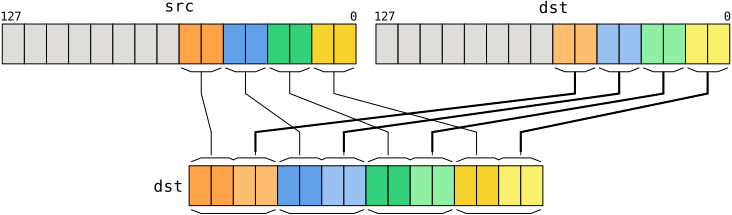
\includegraphics[scale=0.6]{img/inst_unpackl.pdf}} \end{textblock}
    \begin{textblock}{500}(20,49) \only<2>{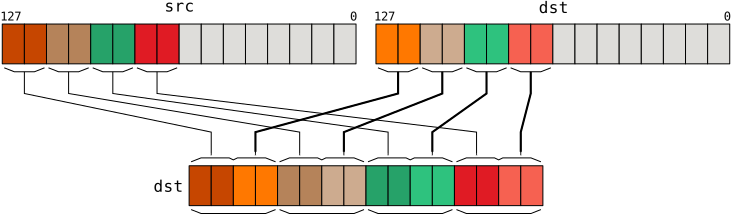
\includegraphics[scale=0.6]{img/inst_unpackh.pdf}} \end{textblock}
    \begin{textblock}{500}(20,74) \only<1>{Low\\  \texttt{PUNPCKLWD}} \end{textblock}
    \begin{textblock}{500}(20,74) \only<2>{High\\ \texttt{PUNPCKHWD}} \end{textblock}
\end{frame}

\begin{frame}[fragile,t]
    \frametitle{Operaciones de desempaquetado (Unpack)}
    \begin{center}
    \begin{tabular}{l|l}
    \hline
    \texttt{PACK\color{a}S\color{y}S\color{v}DW}  & Packs 32 bits (signado) a 16 bits (signado) usando saturation \\
    \texttt{PACK\color{a}U\color{y}S\color{v}DW}  & Packs 32 bits (signado) a 16 bits (sin signo) usando saturation \\
    \texttt{PACK\color{a}S\color{y}S\color{v}WB}  & Packs 16 bits (signado) a 8 bits  (signado) usando saturation \\
    \texttt{PACK\color{a}U\color{y}S\color{v}WB}  & Packs 16 bits (signado) a 8 bits  (sin signo) usando saturation \\
    \hline
    \end{tabular}
    \end{center}
    \begin{textblock}{500}(20,42) \only<1>{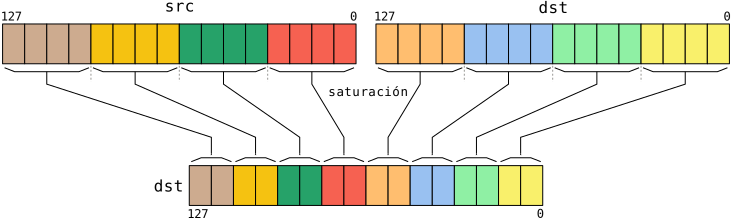
\includegraphics[scale=0.6]{img/inst_pack.pdf}} \end{textblock}
    \begin{textblock}{500}(20,70) \only<1>{\texttt{PACKSSDW} \\ \texttt{PACKUSDW}} \end{textblock}
\end{frame}

% psignd     - Gives 32bit integer magnitudes the sign of the 2nd operand
% psignw     - Gives 16bit integer magnitudes the sign of the 2nd operand
% psignb     - Gives 8bit integer magnitudes the sign of the 2nd operand
% palignr    - Combines two register values, extracts a register value from it, based on an offset
% psadbw     - Returns sum of absolute differences of 8 8bit values Result in bottom 16 bits
% mpsadbw    - Sum of absolute differences
% phminposuw - minimum+index extraction (16bit word)
% dpps       - dot product, single precision
% dppd       - dot product, double precision

\begin{frame}[fragile]
    \frametitle{Técnica: Operatoria de desempaquetado y empaquetado}
    \large
    \begin{textblock}{500}(22,19) \only<1->{\includegraphics[scale=1.4]{img/operation_packunpack-layer1.pdf}} \end{textblock}
    \begin{textblock}{500}(22,19) \only<2->{\includegraphics[scale=1.4]{img/operation_packunpack-layer2.pdf}} \end{textblock}
    \begin{textblock}{500}(22,19) \only<3->{\includegraphics[scale=1.4]{img/operation_packunpack-layer3.pdf}} \end{textblock}
    \begin{textblock}{500}(22,19) \only<4->{\includegraphics[scale=1.4]{img/operation_packunpack-layer4.pdf}} \end{textblock}
    \begin{textblock}{500}(22,19) \only<5-6>{\includegraphics[scale=1.4]{img/operation_packunpack-layer5.pdf}} \end{textblock}
    \begin{textblock}{500}(22,19) \only<6-6>{\includegraphics[scale=1.4]{img/operation_packunpack-layer6.pdf}} \end{textblock}
    \begin{textblock}{500}(22,19) \only<7->{\includegraphics[scale=1.4]{img/operation_packunpack-layer7.pdf}} \end{textblock}
    \begin{textblock}{500}(22,19) \only<8->{\includegraphics[scale=1.4]{img/operation_packunpack-layer8.pdf}} \end{textblock}
\end{frame}

\begin{frame}[fragile]
    \frametitle{Ejemplo}
    \begin{block}{Multiplicar vectores}
    Dado dos vectores de 128 enteros con signo de 16 bits. Multiplicar cada uno de ellos entre si y almacenar el resultado en un vector de enteros de 32 bits.\\
    \bigskip
    \verb|void mulvec(int16_t *v1, int16_t *v2, int32_t *resultado)|
    \end{block}
\end{frame}

\begin{frame}[fragile]
    \frametitle{Multiplicar vectores}
    \scriptsize
    \begin{verbatim}
    mulvec: ; rdi = int16_t *v1, rsi = int16_t *v2, rdx = int32_t *resultado
    push rbp
    mov rbp,rsp
    mov rcx, (128 >> 2) ; rcx = 128 / 8
    \end{verbatim}
    \vspace{-0.8cm} \pause
    \begin{verbatim}
    .ciclo:
        movdqa xmm0, [rdi]    ; xmm0 = | a7 | a6 | a5 | a4 | a3 | a2 | a1 | a0 |
        movdqa xmm1, [rsi]    ; xmm1 = | b7 | b6 | b5 | b4 | b3 | b2 | b1 | b0 |
    \end{verbatim}
    \vspace{-0.8cm} \pause
    \begin{verbatim}
        movdqa xmm2, xmm0     ; xmm2 = | a7 | a6 | a5 | a4 | a3 | a2 | a1 | a0 |
        pmulhw xmm2, xmm1     ; xmm2 = | hi(a7*b7)        ...        hi(a0*b0) |
        pmullw xmm0, xmm1     ; xmm0 = | low(a7*b7)       ...       low(a0*b0) |
    \end{verbatim}
    \vspace{-0.8cm} \pause
    \begin{verbatim}
        movdqa xmm1, xmm0     ; xmm1 = | low(a7*b7)       ...       low(a0*b0) |
        punpcklwd xmm0, xmm2  ; xmm0 = | hi:low(a3*b3)    ...    hi:low(0a*b0) |
        punpckhwd xmm1, xmm2  ; xmm1 = | hi:low(a7*b7)    ...    hi:low(a4*b4) |
    \end{verbatim}
    \vspace{-0.8cm} \pause
    \begin{verbatim}
        movdqa [rdx], xmm0
        movdqa [rdx+16], xmm1
    \end{verbatim}
    \vspace{-0.8cm} \pause
    \begin{verbatim}
        add rdx, 32
        add rdi, 16
        add rsi, 16
    loop .ciclo
    pop rbp
    ret
    \end{verbatim}
\end{frame}

\begin{frame}[fragile]
    \frametitle{Técnica: Operatoria con un kernel}
    \large
    \begin{textblock}{500}(26,15) \only<1->{  \includegraphics[scale=2.1]{img/operation_kernel-layer1.pdf}} \end{textblock} % matriz
    \begin{textblock}{500}(26,15) \only<2->{  \includegraphics[scale=2.1]{img/operation_kernel-layer2.pdf}} \end{textblock} % /16
    \begin{textblock}{500}(26,15) \only<3->{  \includegraphics[scale=2.1]{img/operation_kernel-layer3.pdf}} \end{textblock} % imagen
    \begin{textblock}{500}(26,15) \only<4->{  \includegraphics[scale=2.1]{img/operation_kernel-layer4.pdf}} \end{textblock} % numeros
    \begin{textblock}{500}(26,15) \only<6-6>{ \includegraphics[scale=2.1]{img/operation_kernel-layer5.pdf}} \end{textblock} % matrix 3x3
    \begin{textblock}{500}(26,15) \only<8-8>{ \includegraphics[scale=2.1]{img/operation_kernel-layer6.pdf}} \end{textblock} % procesado
    \begin{textblock}{500}(26,15) \only<5-6>{ \includegraphics[scale=2.1]{img/operation_kernel-layer7.pdf}} \end{textblock} % matrix 3x3 seleccionado
    \begin{textblock}{500}(26,15) \only<7-8>{ \includegraphics[scale=2.1]{img/operation_kernel-layer8.pdf}} \end{textblock} % procesado seleccionado
    \begin{textblock}{500}(26,15) \only<9-18>{\includegraphics[scale=2.1]{img/operation_kernel-layer29.pdf}} \end{textblock} % numeros color
    \begin{textblock}{500}(26,15) \only<10>{  \includegraphics[scale=2.1]{img/operation_kernel-layer9.pdf}} \end{textblock} % 1
    \begin{textblock}{500}(26,15) \only<11>{  \includegraphics[scale=2.1]{img/operation_kernel-layer10.pdf}} \end{textblock} % 2
    \begin{textblock}{500}(26,15) \only<12>{  \includegraphics[scale=2.1]{img/operation_kernel-layer11.pdf}} \end{textblock} % 3
    \begin{textblock}{500}(26,15) \only<13>{  \includegraphics[scale=2.1]{img/operation_kernel-layer12.pdf}} \end{textblock} % 4
    \begin{textblock}{500}(26,15) \only<14>{  \includegraphics[scale=2.1]{img/operation_kernel-layer13.pdf}} \end{textblock} % 5
    \begin{textblock}{500}(26,15) \only<15>{  \includegraphics[scale=2.1]{img/operation_kernel-layer14.pdf}} \end{textblock} % 6
    \begin{textblock}{500}(26,15) \only<16>{  \includegraphics[scale=2.1]{img/operation_kernel-layer15.pdf}} \end{textblock} % 7
    \begin{textblock}{500}(26,15) \only<17>{  \includegraphics[scale=2.1]{img/operation_kernel-layer16.pdf}} \end{textblock} % 8
    \begin{textblock}{500}(26,15) \only<18>{  \includegraphics[scale=2.1]{img/operation_kernel-layer17.pdf}} \end{textblock} % 9
    \begin{textblock}{500}(26,15) \only<10->{ \includegraphics[scale=2.1]{img/operation_kernel-layer18.pdf}} \end{textblock} % caso 1
    \begin{textblock}{500}(26,15) \only<11->{ \includegraphics[scale=2.1]{img/operation_kernel-layer19.pdf}} \end{textblock} % caso 2
    \begin{textblock}{500}(26,15) \only<12->{ \includegraphics[scale=2.1]{img/operation_kernel-layer20.pdf}} \end{textblock} % caso 3
    \begin{textblock}{500}(26,15) \only<13->{ \includegraphics[scale=2.1]{img/operation_kernel-layer21.pdf}} \end{textblock} % caso 4
    \begin{textblock}{500}(26,15) \only<14->{ \includegraphics[scale=2.1]{img/operation_kernel-layer22.pdf}} \end{textblock} % caso 5
    \begin{textblock}{500}(26,15) \only<15->{ \includegraphics[scale=2.1]{img/operation_kernel-layer23.pdf}} \end{textblock} % caso 6
    \begin{textblock}{500}(26,15) \only<16->{ \includegraphics[scale=2.1]{img/operation_kernel-layer24.pdf}} \end{textblock} % caso 7
    \begin{textblock}{500}(26,15) \only<17->{ \includegraphics[scale=2.1]{img/operation_kernel-layer25.pdf}} \end{textblock} % caso 8
    \begin{textblock}{500}(26,15) \only<18->{ \includegraphics[scale=2.1]{img/operation_kernel-layer26.pdf}} \end{textblock} % caso 9
    \begin{textblock}{500}(26,15) \only<19->{ \includegraphics[scale=2.1]{img/operation_kernel-layer27.pdf}} \end{textblock} % resultado
    \begin{textblock}{500}(26,15) \only<19->{ \includegraphics[scale=2.1]{img/operation_kernel-layer28.pdf}} \end{textblock} % resultado
\end{frame}

\begin{frame}[fragile]
    \frametitle{Ejemplo}
    \begin{block}{Efecto Blur}
    Aplicar un kernel de $3 \times 3$ \verb|[[1,2,1],[2,4,2],[1,2,1]] / 16| sobre cada pixel de una imagen de $34 \times 34$ de valores de 8 bits. Almacenar el resultado en una imagen de $32 \times 32$.
    \verb|extern void blur(uint8_t *imgDst, uint8_t *imgSrc)|
    \end{block}
\end{frame}

\begin{frame}[fragile]
    \frametitle{Efecto Blur (Parte 1/5)}
    \footnotesize
\begin{verbatim}
; rdi = uint8_t *imgDst
; rsi = uint8_t *imgSrc

blur:
  push rbp
  mov rbp,rsp
\end{verbatim}
\pause
\begin{verbatim}
  mov rdx, 32          ; rdx = 32 (filas)
  lea rsi, [rsi+34+1]  ; rsi = primera fila mas uno
\end{verbatim}
\pause
\begin{verbatim}
  .cicloFilas:
    mov rcx, 32 >> 3   ; rcx = 32 / 8 (columnas)
\end{verbatim}
\pause
\begin{verbatim}
      .cicloColumnas:
        pxor xmm0, xmm0 ; xmm0 = 0 (acumulador)
\end{verbatim}
\pause
\begin{verbatim}
        ; 1*A 2*D 1*G
        ; 2*B 4*E 2*H
        ; 1*C 2*F 1*I
\end{verbatim}
\end{frame}

\begin{frame}[fragile,t]
    \frametitle{Efecto Blur (Parte 2/5)}
    \small
\begin{verbatim}
        ; 1*A 2*D 1*G
        ; 2*B 4*E 2*H
        ; 1*C 2*F 1*I
\end{verbatim}
\pause
\begin{verbatim}
        pmovzxbw xmm1, [rsi-1-34] ; xmm1 = A
        pmovzxbw xmm2, [rsi-1]    ; xmm2 = B
        pmovzxbw xmm3, [rsi-1+34] ; xmm3 = C
\end{verbatim}
\pause
\begin{verbatim}
        psllw xmm2, 1             ; xmm2 = 2*B
\end{verbatim}
\pause
\begin{verbatim}
        paddw xmm0, xmm1
        paddw xmm0, xmm2
        paddw xmm0, xmm3
\end{verbatim}
\end{frame}

\begin{frame}[fragile,t]
    \frametitle{Efecto Blur (Parte 3/5)}
    \small
\begin{verbatim}
        ; 1*A 2*D 1*G
        ; 2*B 4*E 2*H
        ; 1*C 2*F 1*I
\end{verbatim}
\pause
\begin{verbatim}
        pmovzxbw xmm1, [rsi-34]   ; xmm1 = D
        pmovzxbw xmm2, [rsi]      ; xmm2 = E
        pmovzxbw xmm3, [rsi+34]   ; xmm3 = F
\end{verbatim}
\pause
\begin{verbatim}
        psllw xmm1, 1             ; xmm1 = 2*D
        psllw xmm2, 2             ; xmm2 = 4*E
        psllw xmm3, 1             ; xmm3 = 2*F
\end{verbatim}
\pause
\begin{verbatim}
        paddw xmm0, xmm1
        paddw xmm0, xmm2
        paddw xmm0, xmm3
\end{verbatim}
\end{frame}

\begin{frame}[fragile,t]
    \frametitle{Efecto Blur (Parte 4/5)}
    \small
\begin{verbatim}
        ; 1*A 2*D 1*G
        ; 2*B 4*E 2*H
        ; 1*C 2*F 1*I
\end{verbatim}
\pause
\begin{verbatim}
        pmovzxbw xmm1, [rsi+1-34] ; xmm1 = G
        pmovzxbw xmm2, [rsi+1]    ; xmm2 = H
        pmovzxbw xmm3, [rsi+1+34] ; xmm3 = I
\end{verbatim}
\pause
\begin{verbatim}
        psllw xmm2, 1             ; xmm2 = 2*H
\end{verbatim}
\pause
\begin{verbatim}
        paddw xmm0, xmm1
        paddw xmm0, xmm2
        paddw xmm0, xmm3
\end{verbatim}
\end{frame}

\begin{frame}[fragile]
    \frametitle{Efecto Blur (Parte 5/5)}
    \footnotesize
\begin{verbatim}
        psrlw xmm0, 4
        packuswb xmm0, xmm0
\end{verbatim}
\pause
\begin{verbatim}
        movq [rdi], xmm0
        add rdi, 8
        add rsi, 8
\end{verbatim}
\pause
\begin{verbatim}
      dec rcx
      cmp rcx, 0
      jnz .cicloColumnas
      lea rsi, [rsi+2]
\end{verbatim}
\pause
\begin{verbatim}
  dec rdx
  cmp rdx, 0
  jnz .cicloFilas

  pop rbp
ret

\end{verbatim}
\end{frame}

\begin{frame}[fragile]
    \frametitle{Efecto Blur}
    \scriptsize
    \begin{textblock}{500}(5,10)
    \begin{verbatim}
; rdi = uint8_t *imgDst
; rsi = uint8_t *imgSrc

blur:
  push rbp
  mov rbp,rsp
  
  pxor xmm8, xmm8
  mov rdx, 32
  lea rsi, [rsi+34+1]
  
  .cicloFilas:
    mov rcx, 32 >> 3
    
      .cicloColumnas:
        pxor xmm0, xmm0
        
        ; 1*A 2*D 1*G
        ; 2*B 4*E 2*H
        ; 1*C 2*F 1*I        
\end{verbatim}
    \end{textblock}
    \begin{textblock}{500}(40,0)
    \begin{tikzpicture}[remember picture,overlay]
    \draw (0.7,1) -- (0.7,-9.5);
    \draw (7,1) -- (7,-9.5);
    \end{tikzpicture}
\begin{verbatim}
        pmovzxbw xmm1, [rsi-1-34] ; xmm1 = A
        pmovzxbw xmm2, [rsi-1]    ; xmm2 = B
        pmovzxbw xmm3, [rsi-1+34] ; xmm3 = C
        psllw xmm2, 1             ; xmm2 = 2*B
        paddw xmm0, xmm1
        paddw xmm0, xmm2
        paddw xmm0, xmm3

        pmovzxbw xmm1, [rsi-34]   ; xmm1 = D
        pmovzxbw xmm2, [rsi]      ; xmm2 = E
        pmovzxbw xmm3, [rsi+34]   ; xmm3 = F
        psllw xmm1, 1             ; xmm1 = 2*D
        psllw xmm2, 2             ; xmm2 = 4*E
        psllw xmm3, 1             ; xmm3 = 2*F
        paddw xmm0, xmm1
        paddw xmm0, xmm2
        paddw xmm0, xmm3

        pmovzxbw xmm1, [rsi+1-34] ; xmm1 = G
        pmovzxbw xmm2, [rsi+1]    ; xmm2 = H
        pmovzxbw xmm3, [rsi+1+34] ; xmm3 = I
        psllw xmm2, 1             ; xmm2 = 2*H
        paddw xmm0, xmm1
        paddw xmm0, xmm2
        paddw xmm0, xmm3
\end{verbatim}
    \end{textblock}
    \begin{textblock}{500}(120,10)
\begin{verbatim}

        psrlw xmm0, 4
        packuswb xmm0, xmm0

        movq [rdi], xmm0
        add rdi, 8
        add rsi, 8

      dec rcx
      cmp rcx, 0
      jnz .cicloColumnas
      lea rsi, [rsi+2]

  dec rdx
  cmp rdx, 0
  jnz .cicloFilas

  pop rbp
ret
    \end{verbatim}
    \end{textblock}
\end{frame}

\begin{frame}[fragile]
	\frametitle{Ejercicios}
	\begin{enumerate}
	 \item Sean un vector de 1024 pares de componentes $x$ e $y$, ordenadas una a continuación de la otra. Las componentes están almacenadas en punto flotante de 32 bits. Calcular el módulo del vector que representan utilizando la formula $\sqrt{x^2+y^2}$. Retornar el resultado un nuevo vector. La aridad de la función es \verb|float* mod(float *v)|.
	 \vskip 10pt
	 \item Dados dos vectores de 64 enteros de 16 bits, realizar el producto escalar entre ambos y alamacenar el resultado en 32 bits. La aridad de la función es \verb|int32_t dotProduct(int16_t *a, int16_t *b)|.
	 \vskip 10pt
	 \item Dadas dos matrices de $32 \times 32$ valores en punto flotante de 32 bits, realizar la multiplicación de matrices entre ambas y almacenar el resultado en una nueva matriz solicitando memoria. La aridad de la función es \verb|float* matrixProduct(float *a, float *b)|.
	\end{enumerate}
\end{frame}

\begin{frame}[fragile]
    \frametitle{Bibliografía: Fuentes y material adicional}
    \begin{itemize}
    \item Convenciones de llamados a función en x86: \\
    \url{https://en.wikipedia.org/wiki/X86_calling_conventions}
    \item Notas sobre System V ABI: \\
    \url{https://wiki.osdev.org/System_V_ABI}
    \item Documentación de NASM: \\
    \url{https://nasm.us/doc/}
    \item Artículo sobre el flag \texttt{-pie}: \\
    \url{https://eklitzke.org/position-independent-executables}
    \item Documentación de System V ABI: \\
    \url{https://uclibc.org/docs/psABI-x86_64.pdf}
    \item Manuales de Intel: \\
    \url{https://software.intel.com/en-us/articles/intel-sdm}
    \end{itemize}
\end{frame}

\begin{frame}[plain]
\begin{center}
\vspace{2cm}
\huge ¡Gracias!\\
\vspace{2cm}
\normalsize Recuerden leer los comentarios al final de \\ este video por aclaraciones o fe de erratas.
\end{center}
\end{frame}

\end{document}
